\subsection{Doane 702-Will I get a raise?}
\begin{frame}[t]{Horary: Will I get a raise?}
\begin{columns}[T, onlytextwidth]
\footnotesize
\column{0.5\textwidth}
\Sun\ (L1) averse to 1st, not applying to anyone \\
\Moon\ averse to 1st, applying to \Square\ \Jupiter\ who is \Trine\ 1st \\
\Venus\ (L10) $\Rightarrow$ \Conjunction\ \Saturn \\

\vspace{0.25cm}
The \Sun\ is averse and not applying to another planet that aspects the 1st so can't be used as the significator of the querent. The \Moon\ is also averse but she is applying to \Jupiter\ who is \Trine\ the 1st so the pair can be used. So here, because the \Moon\ is in the 2nd, it can indicate the querent's money and \Jupiter, the querent herself. The aspect indicates an increase but not as much as hoped for as \Jupiter\ is in Fall in \Capricorn. This is further supported by \Jupiter\ applying to conjunct \Saturn\ with reception; possibly indicating her boss (\Saturn\ rules 6th of work and would represent a person of authority) who 'disappoints' as he's in the 12th from the 6th.\\

\vspace{0.2cm}
Looking at \Mercury\ (L2) for her money, he's retro and in Fall in the 7th in opposition to the 1st, and his first application is a \Sextile\ to \Saturn, reinforcing \Jupiter's aspect.\\

\vspace{0.2cm}
The querent did receive a raise but not as much as she had visualized.


\column{0.5\textwidth}
\vspace{-20px}
\begin{center}
{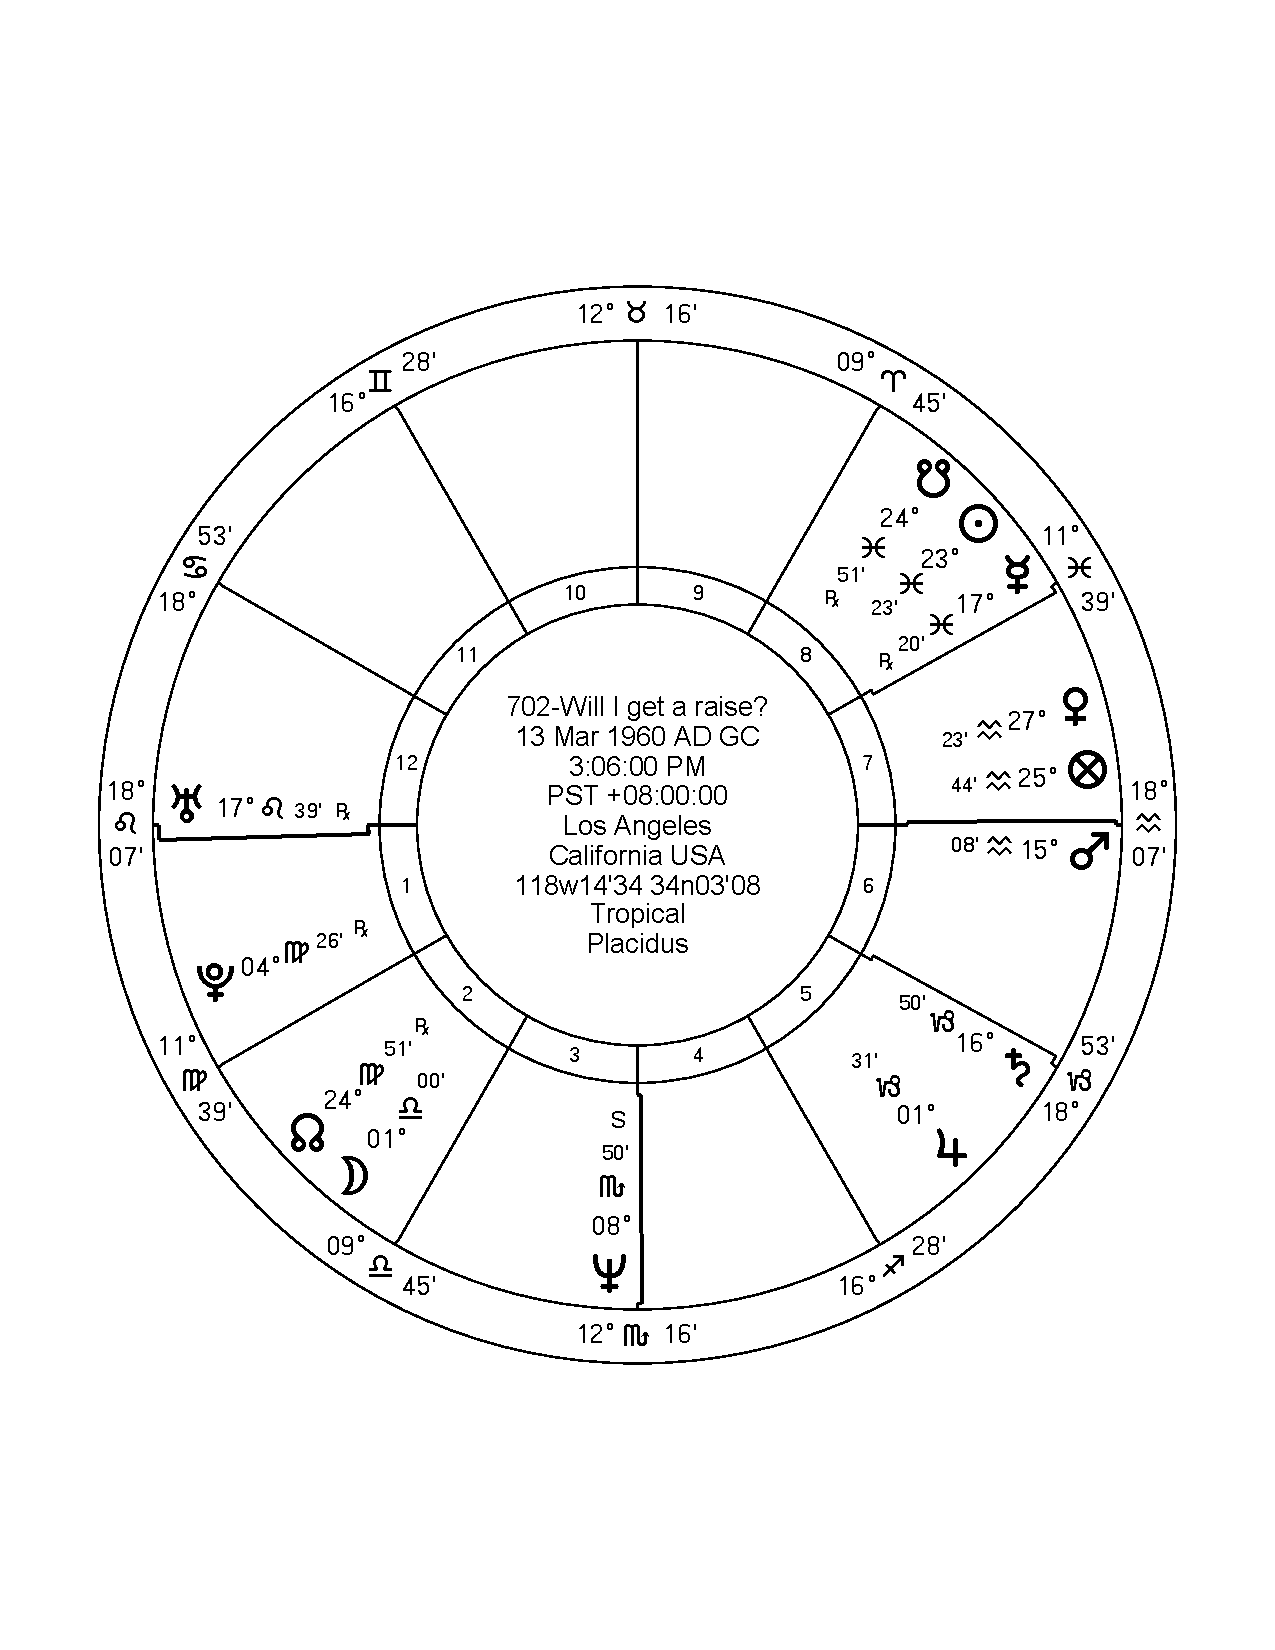
\includegraphics[width=0.9\textwidth]{charts/Doane-702}} \\
\scriptsize
\end{center}
\end{columns}
\scriptsize
Chart from \textsl{Modern Horary Astrology} by Doris Chase Doane, AFA, 1994
\end{frame}